\documentclass{if-beamer}

% --------------------------------------------------- %
%                  Presentation info	              %
% --------------------------------------------------- %
\title[Lecture 6]{Lecture 6}
\subtitle{Random Numbers and Using cmath}
\author{Instructor: Ashley Gannon}
\date{ISC3313 Fall 2021}
\logo{

\includegraphics[scale=0.08]{figures/FSULogo.png}
}
\subject{Presentation subject} % metadata

\graphicspath{{figures/}}
% --------------------------------------------------- %
%                    Title + Schedule                 %
% --------------------------------------------------- %
\begin{document}

\begin{frame}
  \titlepage
\end{frame}
% --------------------------------------------------- %
%                      Presentation                   %
% --------------------------------------------------- %

\section{Random Numbers}

\begin{frame}
\frametitle{Rand class}
\begin{block}{Package}
	$<$stdlib.h$>$
\end{block}
\begin{block}{Usage example}
	int firstRandomNumber = rand();
\end{block}
\begin{block}{Reference}
	http://www.cplusplus.com/reference/cstdlib/rand/
\end{block}

\end{frame}


\begin{frame}
\frametitle{Using the Rand class}
\begin{block}{A random number between 0 and 10?}
int r = rand()\%11;  //Count the numbers in [0, 10] - there are 11
\end{block}
\begin{block}{A random number between 1 and 10?}
int r = rand()\%10 + 1;  //Count the numbers in [1, 10] - there are 10. +1 starts from 1.
\end{block}
\begin{block}{A random number between -10 and 10?}
int r = rand()\%21 - 10; //Count the numbers in [-10, 10] there are 21. -10 starts from -10.
\end{block}
\begin{block}{A random number between 0 and 1? (a decimal number)}
float r = rand() / RAND\_MAX; //RAND\_MAX is the maximum value of rand() 
\end{block}
\end{frame}

\begin{frame}
\frametitle{Using the Rand class}
\begin{block}{A random number between 0 and 10?}
	int r = rand()\%11;  //Count the numbers in [0, 10] - there are 11
\end{block}
\begin{block}{A random number between 1 and 10?}
	int r = rand()\%10 + 1;  //Count the numbers in [1, 10] - there are 10. +1 starts from 1.
\end{block}
\begin{block}{A random number between -10 and 10?}
	int r = rand()\%21 - 10; //Count the numbers in [-10, 10] there are 21. -10 starts from -10.
\end{block}
\begin{block}{A random number between 0 and 1? (a decimal number)}
	float r = rand() / RAND\_MAX; //RAND\_MAX is the maximum value of rand() 
\end{block}

If we compile the same code multiple times, we see that we get the same random number over and over again.
\end{frame}

\begin{frame}
\frametitle{Using the Rand class}
\begin{itemize}
	\item It is not enough to only use the \texttt{rand()} function to make the C++ generate random numbers.\\\vspace{4.5pt}
	\item If you do not use the \texttt{srand} method together with rand, you will get the same sequence every time code runs.\\\vspace{4.5pt}
	\item To avoid the repetitive sequence, you must set the seed as an argument to the \texttt{srand()} method. However, setting a fixed value for the \texttt{srand()} is also not a good option as the output remains the same.\\\vspace{4.5pt}
	\item A very useful tip to make C++ generate random numbers is to use the \texttt{time()} method. By seeding the generator with the same number, you are more likely to get the same random number each time.\\\vspace{4.5pt}
	\item Therefore, if you use the C++ \texttt{srand()} with the current time, the generated random number will always be different.
\end{itemize}

\end{frame}

\begin{frame}
\frametitle{Using the Rand class and the time class}
	\frametitle{Time class}
	\begin{block}{Package}
		$<$ctime$>$
	\end{block}
	\begin{block}{Seeding Rand()}
		srand((unsigned) time(0));
	\end{block}
	\begin{block}{A random number between 0 and 10?}
		srand((unsigned) time(0));\\
		int r = rand()\%11;\qquad \qquad  //Count the numbers in [0, 10] - there are 11
	\end{block}
	\vspace{5pt}
	You can try this with the other examples for practice.
\end{frame}

\section{cmath Basics}

\begin{frame}
	\frametitle{Commands in cmath}
	\begin{block}{Package}
		$<$cmath$>$
	\end{block}
	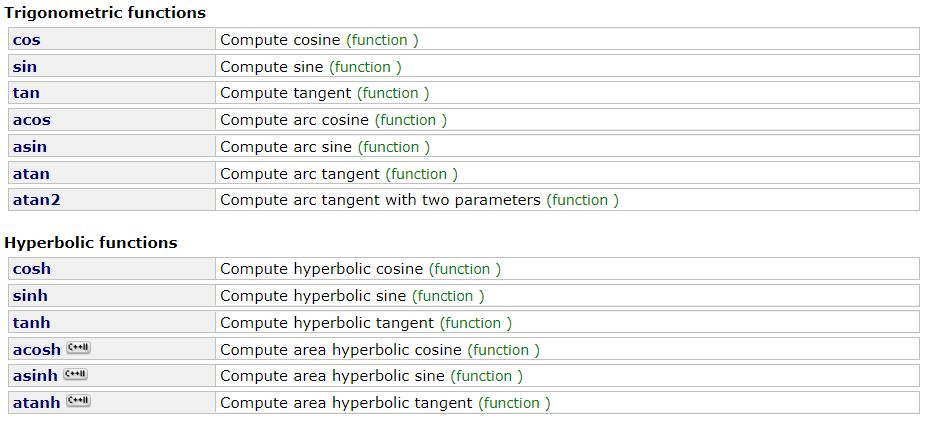
\includegraphics[width = .9\textwidth]{figures/math1}		
\end{frame}

\begin{frame}
\frametitle{Commands in math.h}
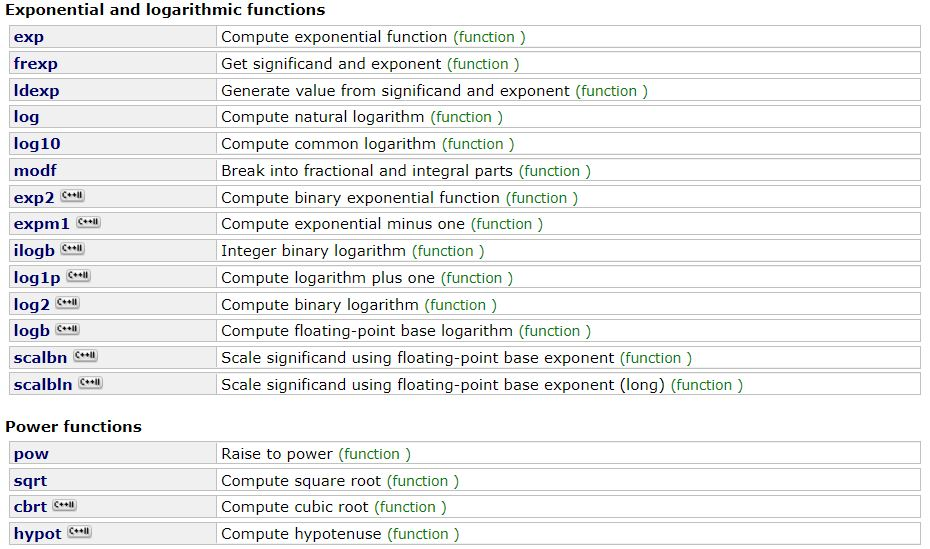
\includegraphics[width = .9\textwidth]{figures/math2} \\
\vspace{5pt}
There are many more! Check out http://www.cplusplus.com/reference/cmath/		
\end{frame}

\section{Class activity}

\begin{frame}
\frametitle{Calculating pi}
\vspace{0.5cm}
In today's activity we are going to write a \texttt{C++} program to
estimate the value of pi using a randomized algorithm. Imagine that we
have a box with dimensions $(0,1)\times(0,1)$, and within it is a circle of
radius 0.5. The areas are then\\
\vspace{1pt}
\begin{minipage}{0.5\textwidth}
	\begin{align*}
	A_{circle} & = \pi r^2 = \pi/4 \\
	A_{square} & = 1 \times 1 = 1.
	\end{align*}
\end{minipage}
\begin{minipage}{0.5\textwidth}
	\flushright
	
\includegraphics[width=.7\textwidth]{figures/circle_box.png}
\end{minipage}
\end{frame}

\begin{frame}
\frametitle{Calculating pi}
Let's imagine that we can throw darts in this domain at random. The
ratio of the darts that land inside the circle to the total should be
the same as the ratio of the area of the circle to the area of the
square. Given coordinates of the `dart' $(x,y)$, we know it lands
inside the circle if
\begin{equation*}
\sqrt{(x-0.5)^2 + (y-0.5)^2} < 0.5
\end{equation*}
\end{frame}

\begin{frame}
\frametitle{Calculating pi}
The number of darts that satisfy this criteria are denoted $N_{hit}$. Then the ratios are equated
as
\begin{equation*}
\frac{A_{circle}}{A_{square}} = \pi (\frac{1}{2})^2 = \frac{\pi}{4} \approx \frac{N_{hit}}{N_{tot}}
\end{equation*}
Then we can compute pi as
\begin{equation*}
\pi \approx 4\frac{N_{hit}}{N_{tot}}
\end{equation*}
\end{frame}

\begin{frame}[shrink=15]
\frametitle{Programming hints}
\vspace{1.5cm}
Please take note of the following: \\\vspace{4.5pt}
\begin{itemize}
\item need to be aware that two integers cannot be used in division
with the expectation of getting a decimal number - Reflect on our \texttt{Types.cpp} code we wrote in class.\\\vspace{4.5pt}
\item must use type-conversion - if we have \texttt{int a} and
\texttt{int b}, convert to double using \texttt{(double) a} 
\texttt{(double) b})\\\vspace{4.5pt}
\item we can use \texttt{\#define} to define constant parameters - you cannot change constant parameters.\\\vspace{4.5pt}
\item we have to seed the random number generator with the line \texttt{srand(time(NULL))}\\\vspace{4.5pt}
\item to get a random number between 0 and 1 use \texttt{((double) rand() / (RAND\_MAX))}
\end{itemize}
\end{frame}

\begin{frame}
\frametitle{Instructions}
Download the file \texttt{computepi.cpp} from Canvas and fill in the
missing code needed to approximate the value $\pi$.
\end{frame}


\end{document}
